\chapter{Mars Entry Phase Guidance Requirements}\label{Ch:EGConcepts}
% High level ideas, feedback concepts. Target conditions, current missions vs future. PHASES - prebank, phase 2 (range control),phase 3 heading alignment 
Figure~\ref{Fig:M2020Timeline} depicts the EDL timeline for the Mars 2020 mission. The entry phase begins when the vehicle enters the atmosphere at 125 km altitude, and ends when the sequence leading to parachute deployment is commanded. 
\begin{figure}[h!]
	\centering
	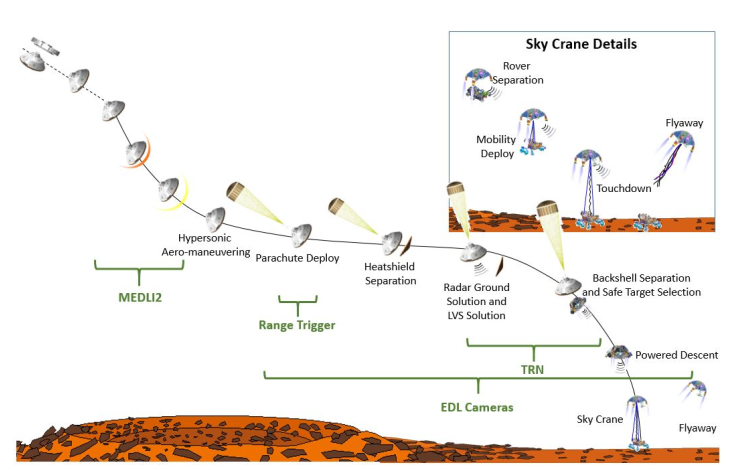
\includegraphics[width=0.95\textwidth]{Images/Mars2020Timeline}
	\caption{Entry Descent and Landing timeline for Mars 2020, taken from~\cite{M2020_EDL}.}
	\label{Fig:M2020Timeline}
\end{figure}
%(landing footprint, deployment within safe parachute deployment conditions, sufficient timeline)
As the discussion of MSL in the introduction highlighted, there are several requirements that entry guidance must meet. 
The vehicle must be delivered to safe parachute deployment conditions, generally given as acceptable ranges of dynamic pressure and Mach number, and the deployment must occur high enough to provide timeline margin for terminal descent. The parachute deploy range dispersion limit is flowed back from the landing footprint requirement. MSL determined that the entry phase had to be terminated within 10 km of the parachute deploy target to achieve the desired touchdown ellipse requirement of 25 x 20 km~\cite{MSL_EDL2}. Mars 2020 had the same touchdown requirement~\cite{M2020_EDL}.
Thus, broadly speaking, the goals are to achieve high terminal altitude and accurate terminal range. 
%Constraints - g-load, heating (handled through selection of mean FPA), and parachute. How are we handling chute? Velocity implies, to an extent, certain mach range. 

\section{Entry Phase Termination}\label{Subsec:EntryTermination}
%Termination of the entry phase
Generally speaking, the entry phase of Mars EDL terminates when the sequence leading to parachute deployment begins. For MSL, this sequence was triggered when the onboard estimated vehicle velocity reached a specified value \cite{MSL_EDL2}. Mars 2020 instead triggered at a fixed downrange distance \cite{TriggerComparison2020}. Future missions, especially those intending to land without the use of a parachute, may consider a different function of the vehicle state \cite{LuAdaptiveEDL,NoyesSRP}. The choice of trigger has a strong impact on the terminal distribution. Naturally, triggering based on the onboard estimated velocity reduces the velocity spread down to approximately the spread in velocity knowledge error. Similarly, a range trigger will naturally minimize the range variations at the trigger point, but will result in larger velocity variations (though the increased to the spread in Mach number is not as large due to wind correlations~\cite{TriggerComparison2020}). We remark that designing entry guidance to reduce range errors is not a moot point in the presence of a range trigger. Large errors in range will turn into large variations in the velocity at which the target range is reached, resulting in Mach variations that may exceed parachute qualification limits.
Regardless of the trigger, the vehicle must meet parachute deployment constraints. Given models of the atmospheric density and local speed of sound on Mars, bounds on the acceptable dynamic pressure and Mach number can be converted into a feasible set in altitude-velocity space. See Fig~\ref{Fig:ParachuteBox} for an example using the Mars 2020 values~\cite{M2020_EDL}, including an additional constraint that the deploy altitude is above 6 km.  
\begin{figure}[h!]
	\centering
	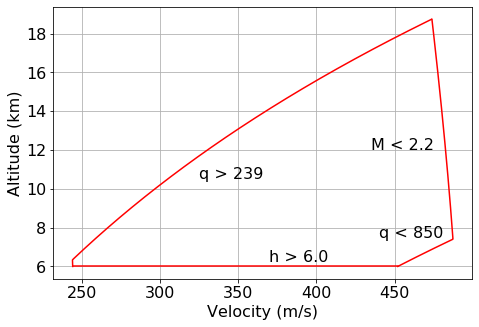
\includegraphics[width=0.75\textwidth]{Images/ParachuteBox}
	\caption{Parachute deployment conditions on Mach number and dynamic pressure in altitude-velocity space.}
	\label{Fig:ParachuteBox}
\end{figure}

One key point is that, despite using different triggers to terminate the entry phase, MSL and Mars 2020 used the same design process involving parametrization of the reference control profile that terminates at a fixed velocity. Together, the control profile and the fixed final velocity define the downrange distance that will be used to trigger the termination of the entry phase in a range trigger design. Thus, the reference design is independent of the trigger used to terminate the entry phase. 
% This the main result/conclusion of this chapter. 
Throughout this dissertation it is assumed the entry phase is terminated based on velocity, using the terminal velocity $v_f=460$ associated with a parachute-based landing, corresponding approximately (because Mach also depends on altitude) to deployment at Mach 2. Like MSL and Mars 2020, the role of the longitudinal entry guidance is to command the vertical lift to steer the vehicle to the the target location at the terminal velocity and with sufficient altitude for subsequent landing operations. We will formalize these objectives, and present the remainder of the problem formulation, in Chapter~\ref{Ch:GuidanceStrategy}.

%Need to say somewhere that reducing range dispersions then using a range trigger, will reduce the velocity (and thus Mach) dispersions. 

%Thus, consistent with designing to an appropriate parachute deployment velocity,
 
%In the event of a different trigger, such as one designed to reduce the propellant consumption required to land at the target location, we assume that a similar process can used. For example, the vehicle would carry a fixed amount of propellant which can be used to null a certain amount of velocity; any velocity under that amount is a candidate to end the entry phase. 

% 


%However, this is not the only possibility. We can, for example, target the velocity at which third phase guidance, such as heading alignment \cite{MSL_EDL2} or final position alignment \cite{GuangfeiDissertation}, begins. 

%Discussion of parachute conditions that we aren't modeling in this phase. The parachute conditions could be included in the assessment conditions. Discussion of parachute-free possibilities? 



%%% Local Variables: ***
%%% mode: latex ***
%%% TeX-master: "thesis.tex" ***
%%% End: ***
